\chapter{Μελέτη της Απόδοσης του VQ H.264}
\label{chapter:chap6}

\section{Εισαγωγή}
\label{section:sect61}

\indent Σε αυτό το κεφάλαιο θα παρουσιαστούν και θα αναλυθούν τα αποτελέσματα του VQ H.264, επίσης θα γίνει σύγκριση με τις επιδόσεις του JM H.264. Επίσης θα δειχθεί ότι με την χρήση VQ μπορούμε να βελτιώσουμε την πολυπλοκότητα του decoder σε σχέση με αυτή του JM H.264.

\section{Encoding με VQ H.264}

\indent Για τις δοκιμές χρησιμοποιήθηκαν 5 βίντεο που δεν είχαν συμπεριληφθεί στο training set και τα στυγμιοτυπα τους φαίνονται στο Σχήμα~\ref{fig:testvid}. Η ποιότητα που αυτά τα βίντεο κωδικοποιήθηκαν φαίνεται στο Σχήμα~\ref{fig:testpsnr}

\begin{table}[h!]
    \begin{center}
        \begin{tabular}{| l | l | l | l |}
        \hline
        Test Video & PSNR I (Y/U/V)dB  & PSNR P (Y/U/V)dB  & PSNR B (Y/U/V)dB       \\ \hline
        test1      & 35.15/39.72/39.67 & 41.16/43.91/43.87 & 43.00/45.14/45.22      \\ \hline
        test2      & 35.51/41.10/42.83 & 38.87/41.53/43.28 & 40.38/43.01/44.71      \\ \hline
        test3      & 30.70/39.86/41.00 & 36.68/42.64/43.76 & 38.00/43.74/44.90      \\ \hline
        test4      & 44.12/47.36/47.91 & 46.00/47.20/47.75 & 46.55/47.42/48.05      \\ \hline
        test5      & 37.01/50.12/48.70 & 44.00/49.90/49.65 & 44.78/50.46/50.29      \\ \hline
        \hline
        \end{tabular}
    \end{center}

    \caption{PSNR of Test videos with VQ H.264}
    \label{table:trainingset}
\end{table}

\begin{table}[h!]
    \begin{center}
        \begin{tabular}{| l | l | l | l |}
        \hline
        Test Video & I bits  & P bits  & B bits       \\ \hline
        test1      &  &  &       \\ \hline
        test2      &  &  &       \\ \hline
        test3      &  &  &       \\ \hline
        test4      &  &  &       \\ \hline
        test5      &  &  &       \\ \hline
        \hline
        \end{tabular}
    \end{center}

    \caption{codebooks}
    \label{table:avgdata}
\end{table}

\begin{figure}[p]
\centering
\begin{tabular}{c c}
    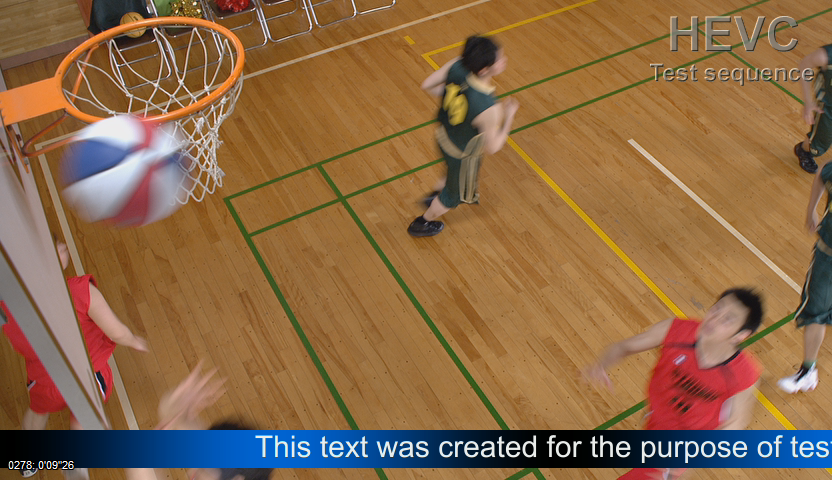
\includegraphics[height=4.0cm]{chapter6/test1.png}
    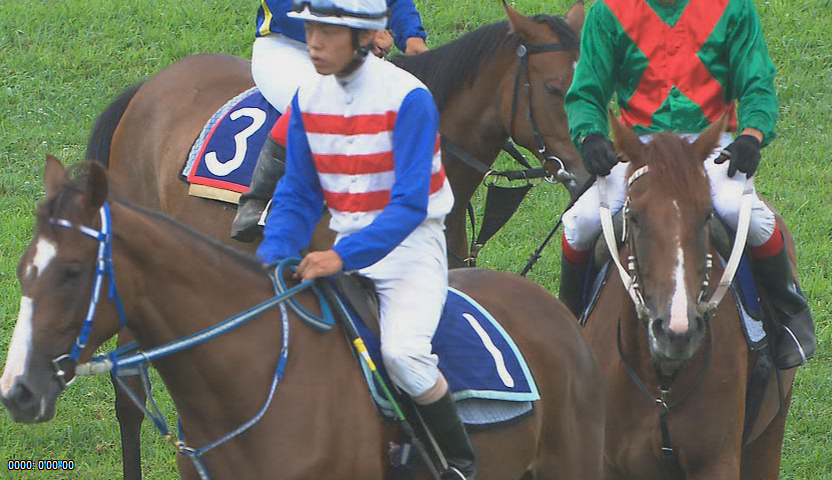
\includegraphics[height=4.0cm]{chapter6/test2.png}\\
    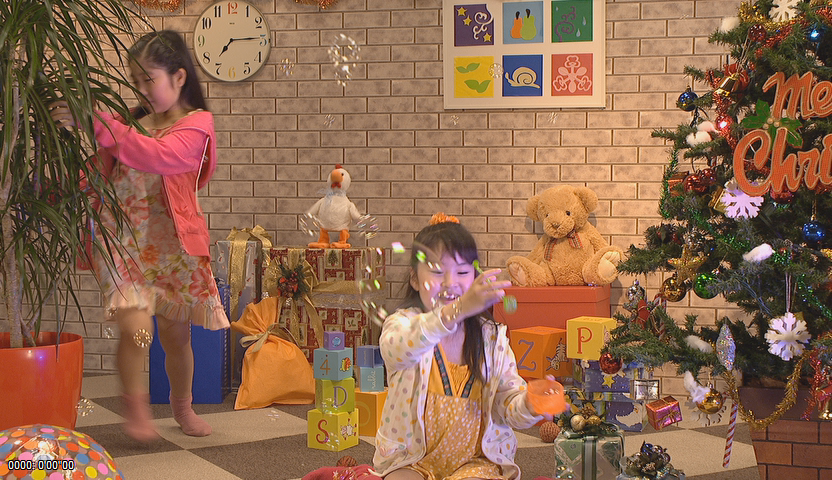
\includegraphics[height=4.0cm]{chapter6/test3.png}
    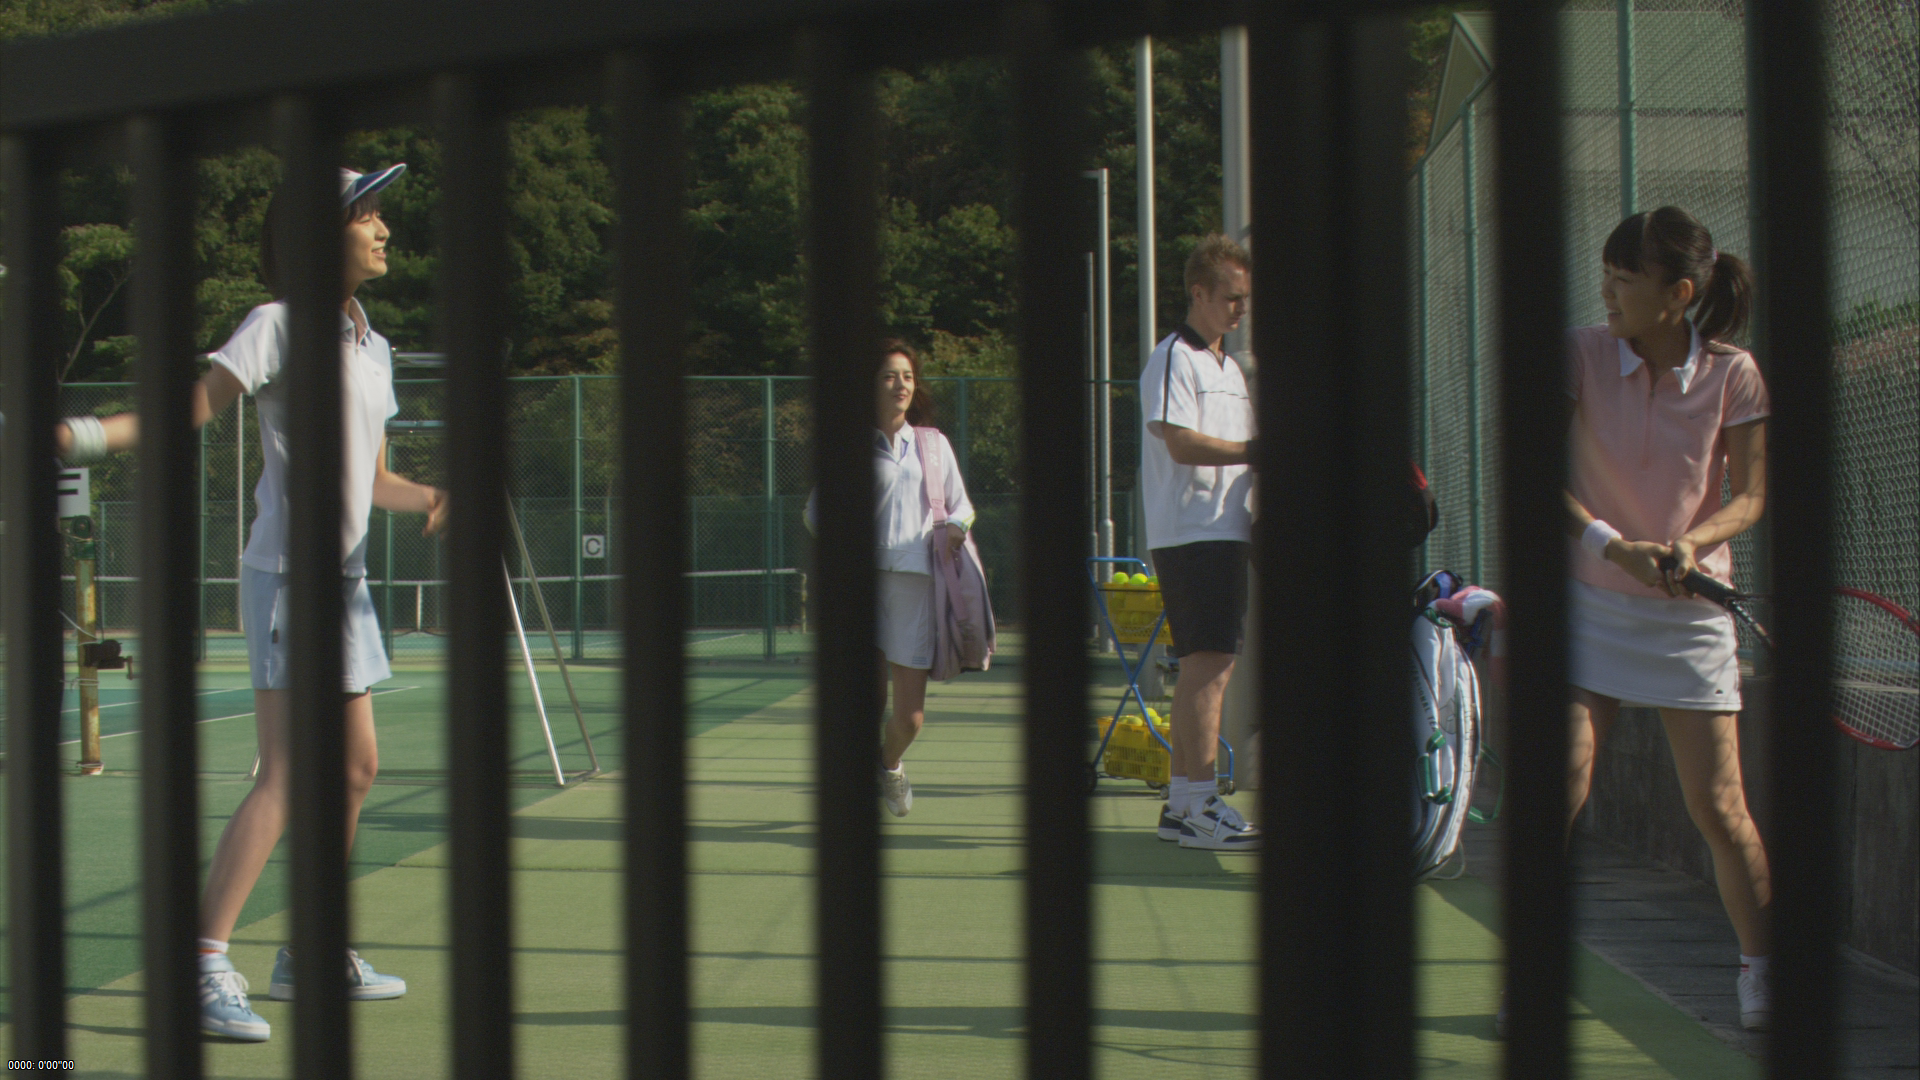
\includegraphics[height=4.0cm]{chapter6/test4.png}\\
    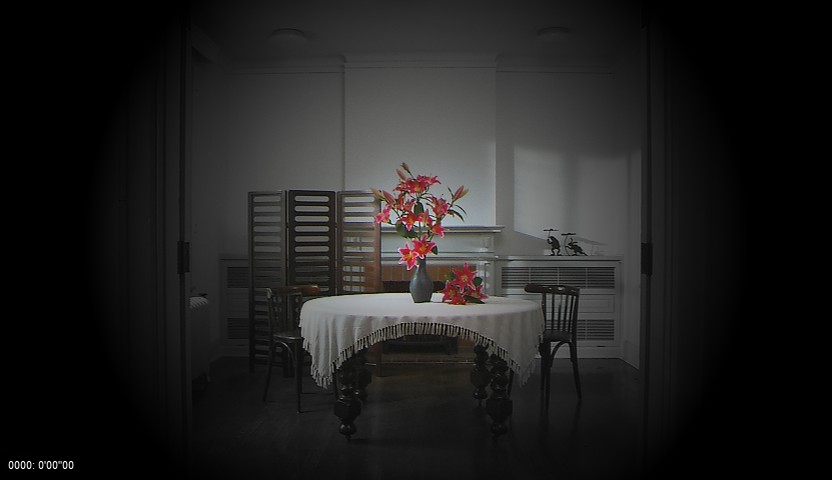
\includegraphics[height=4.0cm]{chapter6/test5.png}
\end{tabular}
\caption{Βίντεο που δοκιμάστηκαν να γίνουν encoding με τον VQ H.264.}
\label{fig:testvid}
\end{figure}


